\graphicspath{{images/}}

\section{\thesection~Results}
\label{sec:results}


% \subsection{\thesubsection~Guessing}
% \end{multicols}
% \graphicspath{{images/guessing/}}
% \begin{Figure}
%   \centering
%   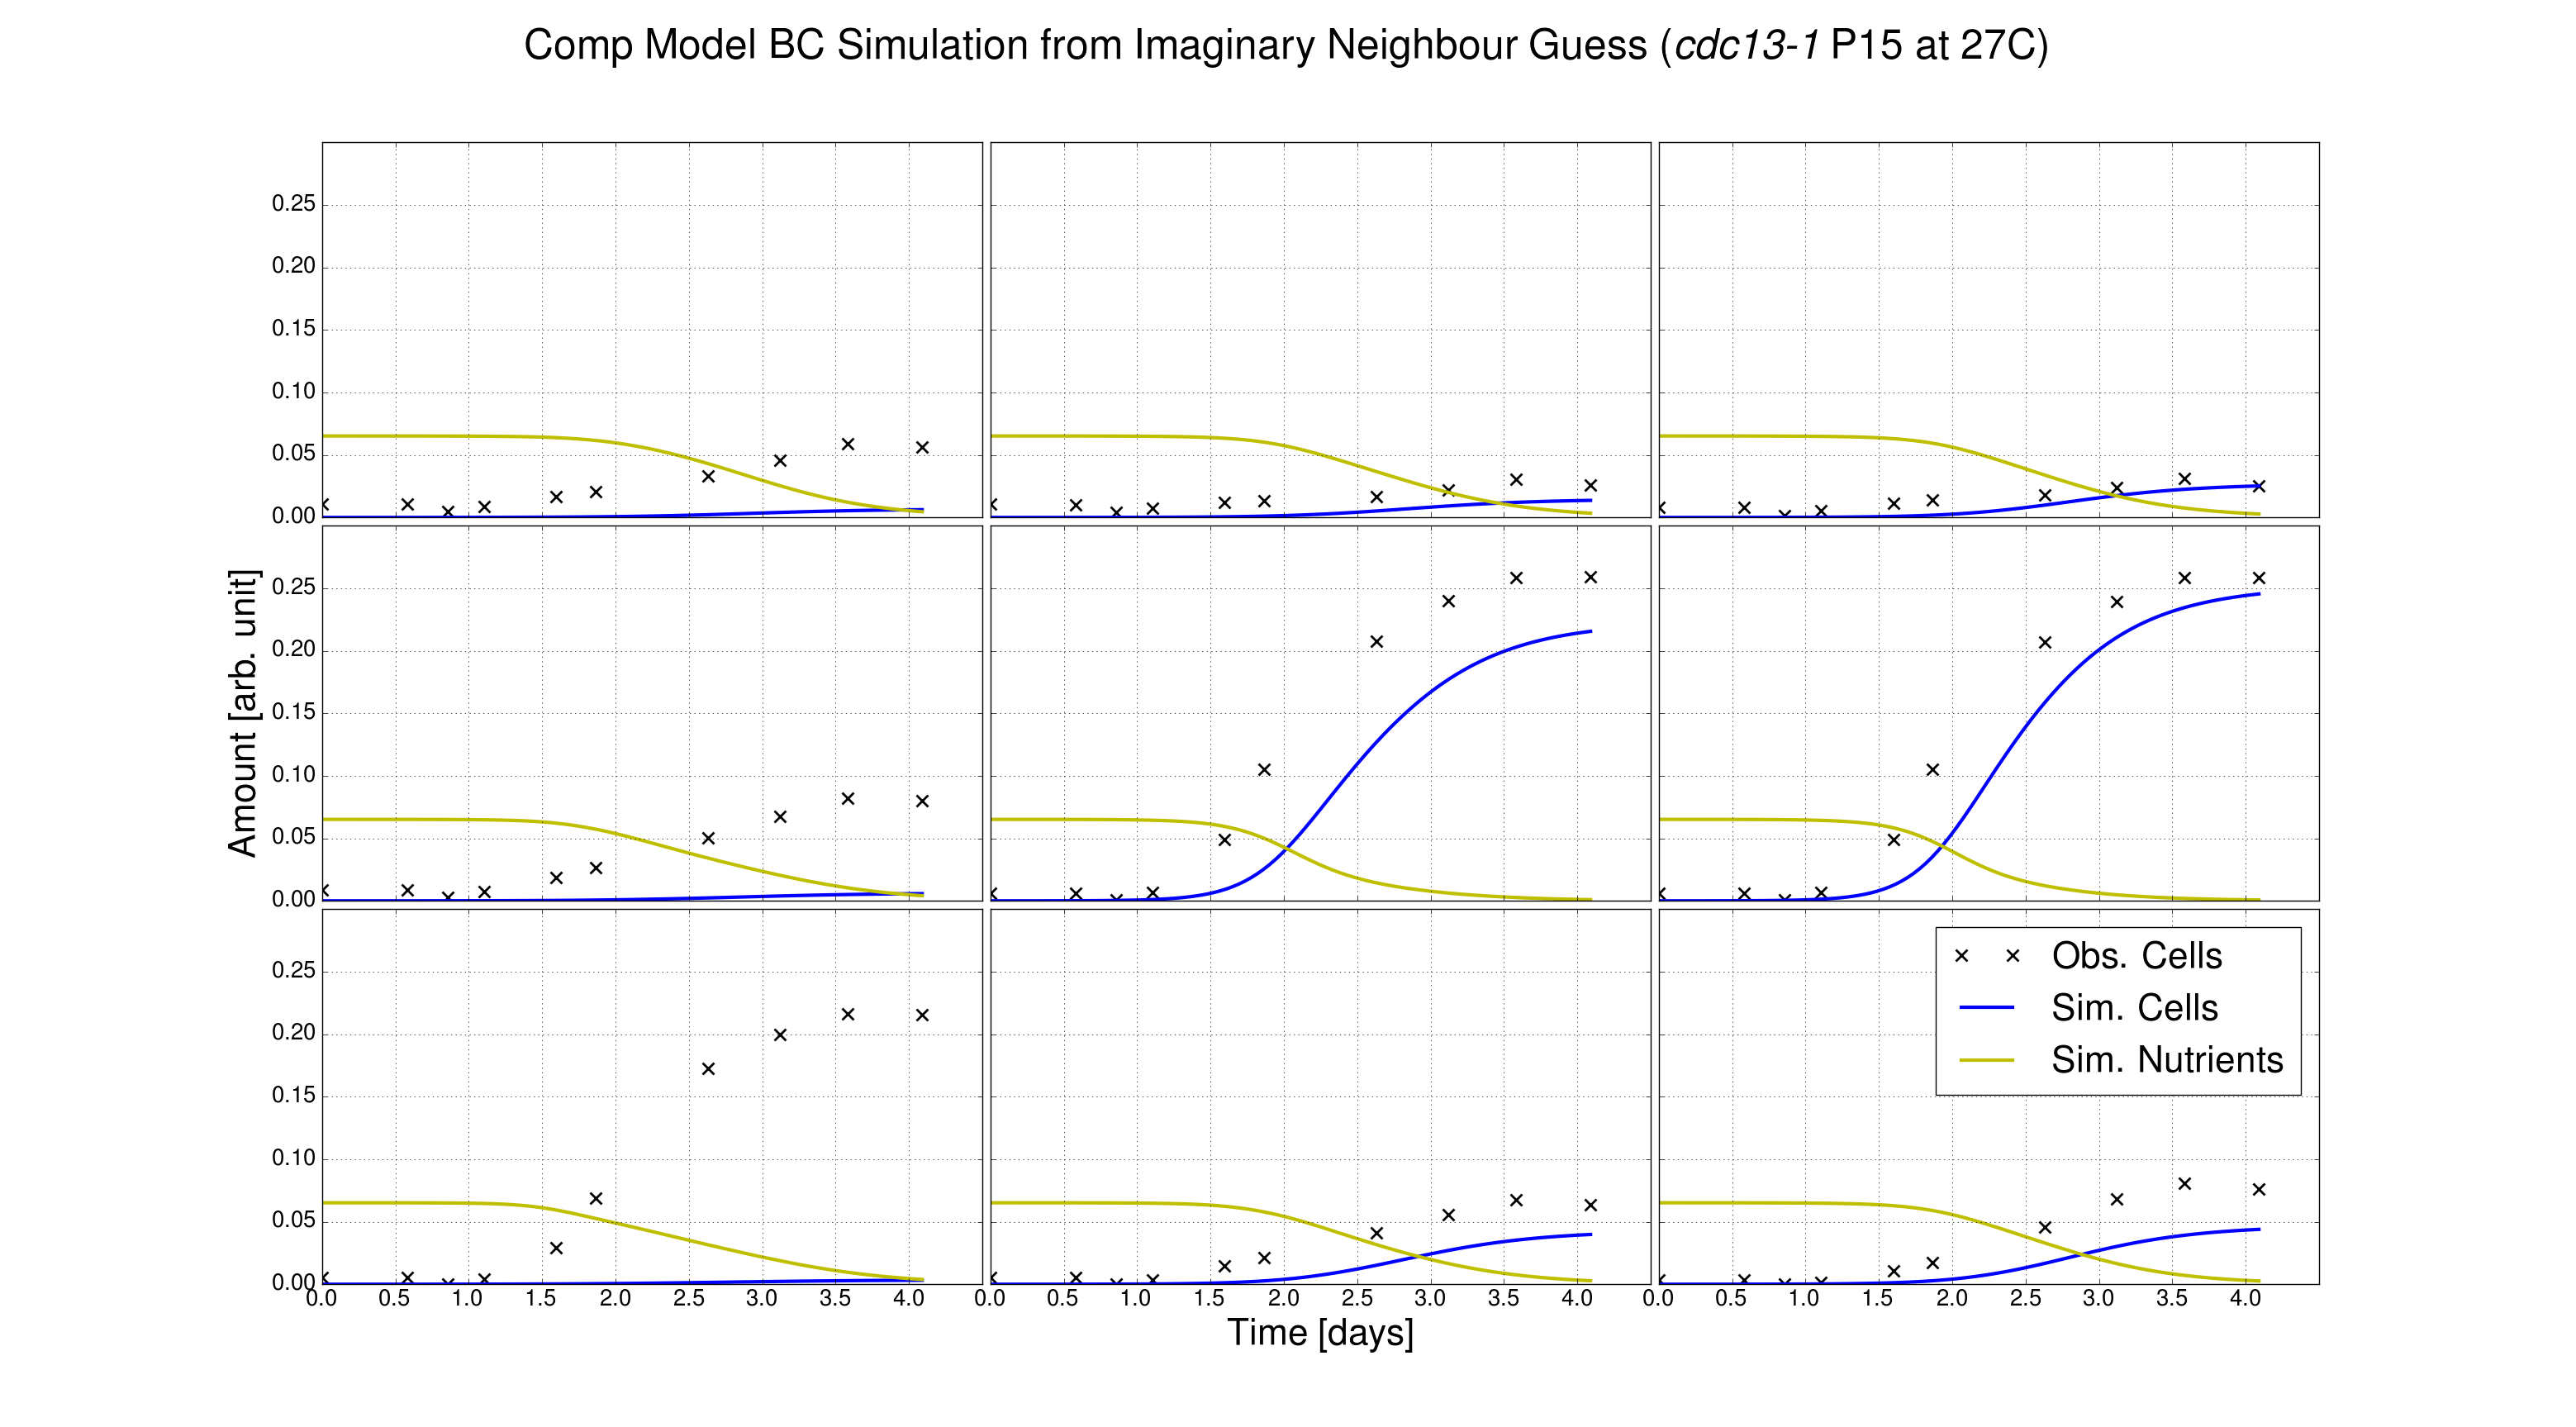
\includegraphics[width=\linewidth]{final/P15_R5_C18_guess_sim}
%   \captionof{figure}{\textbf{Competition model simulation using
%       parameters from imaginary neighbour guessing.} Shows a 3x3 zone
%     with top-left coordinate (5, 18) from P15 with background
%     \textit{cdc13-1} at 27\(^{\circ}C\).}
%   \label{fig:imag_neigh_guess_sim}
% \end{Figure}
% \begin{multicols}{2}

% Scripts were run with combinations of the following values.
% cellratios = np.logspace(-3, -5, num=5)
% fittype = ["imagneigh", "logeq"]
% zerokn = [True, False]

% Each script looped through the following array of b values which were
% supplied to the initial guesser and used at the plate level.

% for b-guess in [35, 40, 45, 50, 55, 60, 65, 70, 75, 80, 95, 100, 150]:

\subsection{\thesubsection~Model comparison using P15}
\label{sec:P15_fit}

I ran multiple fits of the competition model to P15 (see
Section~\ref{sec:P15_description}). Each fit used the imaginary
neighbour model to make initial parameter guesses (see
Section~\ref{sec:guessing_b}. The imaginary neighbour model itself
requires initial parameters and fits looped over combinations of
values for initial cell density \(C(0)\) and growth constant \(b\). I
used five initial values of \(C(0)\) ranging from
\(N(0)\times\)10\(^{-5}\) to \(N(0)\times\)10\(^{-3}\) in logspace
(\(N(0)\) is approximately equal to final cells) and a range of 14
different values for \(b\) as described in
Section~\ref{sec:guessing_b}. This made a total of 70 fits. I show
estimated competition model parameters for the top two fits in
Table~\ref{tab:P15_best_fit_params}. (I selected the best fit based on
the fit to only the internal cultures.) Estimated initial nutrient
amounts agree fairly well between the top two fits but there is
disagreement in estimates of \(C(0)\) and (nutrient diffusion
constant) \(k\). It appears that the gradient method is not finding a
global minimum. However, \(b_{i}\) estimates were correlated with
Spearman's rank correlation coefficient, \(\rho_{S} = 0.989\), and had
average mean absolute deviation, \(MAD = 1.56\). The mean value of
\(b_{i}\) for the best fit was 44.4 so the disagreement is fairly
small.

For all comparisons between the top four fits \(\rho_{S}\) ranges from
0.922 to 0.995 and \(b\) MAD ranges from 1.56 to 6.90. I discarded the
5th best fit, which has less agreement, because, unlike the other
fits, it estimated \(N_{I}(0)\) > \(N_{E}(0)\). When comparing to the
top four fits, \(\rho_{S}\) was above 0.930 but \(b\) values were more
affected with a maximum MAD of 13.29. Despite not finding a global
minimum, the best competition model estimates agree well enough with
each other to make meaningful comparison with logistic model
estimates.


\begin{center}
  \captionof{table}{\textbf{Estimated parameter values for the best
      two competition model fits to P15.} Spearman's rank correlation
    coefficient between \(b_{i}\) estimates, \(\rho_{S}\) =
    0.989. Mean absolute deviation between \(b_{i}\) estimates, MAD =
    1.56. The total objective function value for internal cultures is
    shown in the last column (lower is better).}
  \begin{tabular}{l l l l l l}
    \hline
    Fit     & \(C(0)\)                    & \(N_{I}(0)\) & \(N_{E}(0)\) & \(k\) & Obj.\\
    \hline
    1st     & 9.1\(\times\)10\(^{-5}\)    & 0.064      & 0.090       & 6.7  & 0.194 \\
    2nd     & 13.9\(\times\)10\(^{-5}\)   & 0.062      & 0.097       & 8.3  & 0.196 \\
    \hline
  \end{tabular}
  \label{tab:P15_best_fit_params}
\end{center}


%%%%
\graphicspath{{images/p15_fits/}}
\begin{Figure}
  \centering
  \includegraphics[width=\linewidth]{final/zone_r5_c18_with_obj_fun}
  \captionof{figure}{\textbf{Comparison of competition and logistic
      model fits to a zone of P15}. The logistic model was fit with
    the QFA R package and uses almost three times as many
    parameters. The initial guess (dashes) for the competition model
    was made from fits of the imaginary neighbour model to individual
    cultures. The zone has top-left coordinates (5, 18) and is boxed
    in red in Figure~\ref{fig:comp_fit_plate}. Objective function
    values for each culture (Obj.) were scaled by \(10^{4}\) (smaller
    values are better)}
  \label{fig:P15_zone_fit}
\end{Figure}


For the best fit of the competition model to P15, estimated cell
amounts (blue) match the data well across the entire plate
(Figure~\ref{fig:comp_fit_plate}). A high nutrient diffusion constant,
\(k\), is fit, such that nutrients diffuse readily and nutrient
timecourses are similar in local areas of the plate. Fits of the
competition model (solid), imaginary neighbour guess (dashed), and
logistic model (red) are plotted for a 3x3 zone in
Figure~\ref{fig:P15_zone_fit}. The logistic model was fit using the
QFA R package \citep{qfa2016}. The fit of the initial guess is typical
for the plate. Some culture, such as the bottom-left, are not well fit
(and Spearman's \(\rho_{s}\) for the imaginary neighbour guess and
competition model \(b_{i}\) estimates is 0.63). However, the guess
fulfils its purpose by leading to a good fit when used to initialise
parameters of the competition model. Over the plate, the logistic
model fits slightly better than competition model
(Table\ref{tab:P15_obj_fun}). To make objective function comparisons
fair, I converted logistic model parameters to competition model
parameters (\ref{eq:conversion}) and resimulated both models using
CANS. I discarded edge cultures which have higher noise. The total
objective function for internal cultures is 0.155 for the logistic
model and 0.194 for the competition model (smaller values are
better). (However, the logistic model used 1152 parameters whereas the
competition model only used 387.) The zone in
Figure~Figure~\ref{fig:P15_zone_fit} contains more fast growing
cultures than is typical for the plate (and may contain more
competition effects). The objective function of the logistic and
competition model fit is similar for most cultures. However, the
competition model fits the centre and centre-right fast growing
cultures much better than the logistic model. The total objective
function value for the zone is lower for the competition model: 44.06
vs 68.38 (values scaled by \(10^{4}\)). The logistic model must
provide the better fit for other areas of the plate.

\begin{center}
  \captionof{table}{\textbf{Objective function values for fits to
      P15.} ``Internal'' is the total objective function value for
    cultures not at an edge. ``All'' is the total objective function
    value for all cultures on the plate. Smaller values are better.}
  \begin{tabular}{l l l}
    \hline
    Cultures     & Competition & Logistic \\
    \hline
    Internal     & 0.194    & 0.155\\
    All          & 0.465    & 0.345\\
    \hline
  \end{tabular}
  \label{tab:P15_obj_fun}
\end{center}

\subsection{\boldmath \thesubsection~Correlation or \(r\) estimates between models \unboldmath}

I converted competition model estimates of \(b_{i}\) to logistic model
\(r_{i}\) using (\ref{eq:conversion}). I took the median \(r\) for
each deletion for both the competition and logistic model. I took the
median, rather than mean, to reduce the effect of outliers that may
results from cross-contamination of strains or inoculation with dead
cells. Figure~\ref{fig:P15_correlations} shows correlations, between
models, of estimates for each culture (black) and of median estimates
for each deletion (red). The distribution for cultures is split into
two distinct correlated groups. This is due to a gap in the
distribution of logistic model \(r\) at around \(r\) = 4. There is no
such gap in the distribution of competition model \(r\). The groups
only overlap for medium values of competition model \(r\)
estimates. The larger group, with lower logistic model \(r\), is
correlated with competition model \(r\) with gradient close to
one. However, competition model estimates were lower for almost all
cultures. In the outlying group, competition model \(r\) varies more
steeply with logistic model \(r\).

There are several extreme outliers in the correlation between
cultures. The QFA R package uses heuristic checks to correct for
confounding between \(r\) and \(K\) estimates for slow growing
cultures. These are required becuase cultures are fit individually and
slow growing cultures contain more noise. For the eight outliers on
the left axis, the checks set \(r\) = 0. The two outliers with very
high logistic \(r\) are repeats of \textit{rad50\(\Delta\)} and
\textit{est1\(\Delta\)}. They have escaped the heuristic checks and
exhibit the confounding effect between \(r\) and \(K\).

In the distribution of the medians (red), most deletions fall inside
the main group of cultures with lower logistic \(r\). There are also
several deletions with high competition model \(r\) that fall inside
the outlying group (top-right). A significant number of deletions lie
in the region between the two groups meaning that repeats of these
cultures are split between the two groups. This worsens the
correlation of \(r\) ranks between deletions compared to cultures.
Spearman's rank correlation coefficient, \(\rho_{S}\), measures the
correlation between rank orders of two variables. A monotonic function
has a value of 1 or -1. Other correlations fall between these
values. For cultures \(\rho_{S}\) = 0.731, for deletions \(\rho_{S}\)
= 0.497. (\(\rho_{S}\) is improved when comparing competition model
\(b\), or equivalently \(MDR\), with logistic model \(MDR\) (see
Figure~\ref{fig:comp_vs_log_ranking}).)

\graphicspath{{images/p15_correlations/}}
\begin{Figure}
  \centering
  \includegraphics[width=\linewidth]{final/r_correlations_median_spearmans_trimmed}
  \captionof{figure}{\textbf{Correlation between logistic and
      competition model r estimates for P15}. Correlations are plotted
    between r estimates for each culture (black) and between medians
    of r estimates for each deletion (red). There were six repeats in
    random locations per deletion (except for the neutral deletion
    \textit{his3\(\Delta\)} which had 14). Logistic fits used the QFA
    R package. Spearman's rank correlation coefficient, \(\rho_{s}\),
    is shown for each distribution. The line y = x is also plotted.}
  \label{fig:P15_correlations}
\end{Figure}

\subsection{\thesubsection~Comparison of fitness ranking}

%%%% Write here

In Figure~\ref{fig:comp_vs_log_ranking}, I compare deletions on P15
ranked by competition model \(b\), logistic model \(r\), and logistic
model \(MDR\). The fittest deletions are at the topT. For each fitness
measure, I took the median estimate from repeats of each deletion. I
used the QFA R package to infer logistic model \(r\) and \(MDR\) and
\(b\) from the best fit of the competition model. Competition model
\(b\), \(r\), and \(MDR\) rank are equivalent (see
Section~\ref{sec:parameter_conversion}) so it is not necessary to
convert \(b\) to comparing rankings.

Logistic model \(r\) and \(MDR\) rankings agree for all but two
deletions: \textit{rad50\(\Delta\)} and \textit{est1\(\Delta\)}. These
are the same deletions as the two outliers with high logistic model
\(r\) values in Figure~\ref{fig:P15_correlations}. When \(MDR\) is
calculated (\ref{eq:MDR_MDP}a), the confounding between \(r\) and
\(K\) is corrected for and the rank of these deletions agrees well
with competition model \(b\) rank. As a result, Spearman's
\(\rho_{S}\) is higher for competition model \(b\) and logistic model
\(MDR\) (0.635) than it was for competition model \(b\) and logistic
model \(r\) (0.497). When comparing competition model \(b\) rank with
logistic model \(MDR\) rank, there is good agreement between the
extreme rankings but middle rankings appear almost inverted. There is
a disagreement of 13 places in the rank of the neutral deletion
\textit{his3\(\Delta\)}.

\graphicspath{{images/rank/}}
\begin{Figure}
  \centering
  \includegraphics[width=\linewidth]{final/median_ranks_comp_b_log_r_MDR}
  \captionof{figure}{\textbf{Comparison of \(\bm{r}\) ranking for fits
      of the competition and logistic model to P15.} Rankings are
    determined from median parameter estimates for repeats of each
    deletion. Logistic \(r\) and \(MDR\) were inferred using the QFA R
    package which makes heuristic checks for slow growing cultures.
    For competition \(b\) and logistic \(r\), Spearman's
    \(\rho_{S} = 0.497\); for competition \(b\) and logistic \(MDR\),
    Spearman's \(\rho_{S} = 0.635\). \textit{his3\(\Delta\)} (bold) is
    a neutral deletion.}
  \label{fig:comp_vs_log_ranking}
\end{Figure}


% \graphicspath{{images/rank/}}
% \begin{Figure}
%   \centering
%   \includegraphics[width=\linewidth]{final/comp_b_log_r_trimmed}
%   \captionof{figure}{\textbf{Comparison of \(\bm{r}\) ranking for fits
%       of the competition and logistic model to P15.} Fitnesses of
%     genetic strains are ranked most to least fit from top to
%     bottom. Competition model \(r\) was converted from \(b\), \(N_0\),
%     and \(C_0\) from the best competition model estimate. Logistic
%     \(r\) and \(MDR\) were taken from logistic model fits using the
%     QFA R package which makes heuristic checks for slow growing
%     cultures.}
%   \label{fig:comp_vs_log_ranking2}
% \end{Figure}



% Complicated correlation coefficient table
% \columnbreak
% \begin{center}
%   \captionof{table}{\textbf{Correlation coefficients between logistic
%       and competition model estimates of parameters for P15.} Pearson
%     correlation coefficient \(\rho\) and Spearman rank correlation
%     coefficient \(r_{s}\) are shown. Correlation coefficients compare
%     between logistic and competition model estimates for both \(r\)
%     and \(MDR\). Correlations are shown between estimates for each
%     culture and between median and mean estimates for each deletion.}
% \begin{tabular}{ |c|c|c|c|c| } \cline{2-5}
% \multicolumn{1}{c|}{} & \multicolumn{2}{c|}{\(r\)} & \multicolumn{2}{c|}{\(MDR\)}\\ \hline
% \multicolumn{1}{|c|}{Estimates} & \(\rho\) & \(r_{s}\) & \(\rho\) & \(r_{s}\)\\ \hline
% Culture & 0.712 & 0.731 & 0.752 & 0.754\\
% Median & 0.708 & 0.497 & 0.791 & 0.635\\
% Mean   & 0.763 & 0.594 & 0.885 & 0.732\\ \hline
% \end{tabular}
% \end{center}

% Just a fit of a zone
% \end{multicols}
% \graphicspath{{images/comp_fit/}}
% \begin{Figure}
%   \centering
%   \includegraphics[width=\linewidth]{final/P15_guess_and_fit_r5_c18}
%   \captionof{figure}{\textbf{A zone of a fit of the competition model
%       to P15 and initial guess}. The guess was made using the
%     imaginary neighbour model fit to individual cultures. Top-left
%     coordinates from Figure~\ref{fig:comp_fit_plate} (5, 18).}
%   \label{fig:comp_fit_zone_old}
% \end{Figure}
% \begin{multicols}{2}





% Make landscape and take a whole page.
\end{multicols}
\begin{landscape}
\graphicspath{{images/comp_fit/}}
\begin{Figure}
  \centering
  \includegraphics[width=\linewidth]{full_plate/final/P15_12x20}
  \captionof{figure}{\textbf{Fit of the competition model to P15.}
    Data is for a 16x24 format plate (P15) with a background mutation
    \textit{cdc13-1} incubated at 27\(^{\circ}C\). The plate contains
    6 repeats of 50 genetic strains randomly arranged across the
    internal cultures. Repeats of a single strain are used for all
    edge cultures (removed in the plot). Model output for state
    variable, cell population size (blue curve), is fit to observed
    data (black crosses). Model predictions for unobserved variable
    (nutrient amount) are also plotted (yellow).}
  \label{fig:comp_fit_plate}
\end{Figure}
\end{landscape}
\begin{multicols}{2}



\subsection{\thesubsection~Evaluating the treatment of boundaries}

I also fit the one \(N(0)\) parameter competition model to P15 using
the same method as for the two \(N(0)\) parameter model (see
Section~\ref{sec:P15_fit}). Fits appear similar in quality for both
models (Figure~\ref{fig:P15_corner}) and objective function values for
the entire plate are very similar (Table~\ref{tab:corner}). Objective
function values for cultures next to an edge culture are improved with
the two \(N(0)\) model and internal cultures were better fit
overall. Interestingly, fits of the edge cultures are actually worse
in the two \(N(0)\) model. These cultures are dominated by noise due
to reflections from plate walls which is why they are discarded from
final estimates. However, the edge cultures must be included in the
objective function when fitting the competition model. Despite this
deficit, the two \(N(0)\) model has increased the goodness of fit to
internal cultures by collectively fitting all cultures.


\graphicspath{{images/corners/}}
\begin{Figure}
  \centering
  \includegraphics[width=\linewidth]{final/top_left_new_aspect}
  \captionof{figure}{\textbf{Treatment of boundary conditions in fits
      of the competition model.} The top left corner of a 16x24 QFA
    plate fitted with two versions of the competition model, the first
    has a single initial nutrient amount for all cultures, the second
    has a separate initial nutrient amount for edge cultures.}
  \label{fig:P15_corner}
\end{Figure}


\begin{center}
  \captionof{table}{\textbf{Average objective function value for one a
      two \(\bm{N(0)}\) parameter competition models.} Values are for
    the same fits as in Figure~\ref{fig:P15_corner} and have been
    scaled by \(10^{4}\). Averages are for cultures belonging to the
    areas indicated by the column ``Cultures''. ``Next to edge''
    refers to cultures one in from the edge. ``Internal'' refers to
    all cultures but the edge. Lower values are better.}
  \begin{tabular}{l l l}
    \hline
    Cultures     & One \(N(0)\)  & Two \(N(0)\) \\
    \hline
    Edge         & 35.9    & 36.5\\
    Next to edge & 9.54    & 7.98\\
    Internal     & 6.67    & 6.30\\
    All          & 12.4    & 12.2\\
    \hline
  \end{tabular}
  \label{tab:corner}
\end{center}



% \subsection{\thesubsection~Agreement of b rankings}

%   text Some text Some text Some text Some text Some text Some text
%   Some text Some text Some text Some text.
% \graphicspath{{images/rank/}}
% \begin{Figure}
%   \centering
%   \includegraphics[width=\linewidth]{top_two_comp_p15_correlations_trimmed}
%   \captionof{figure}{\textbf{Comparison of \(\bm{b}\) ranking for the
%       best five competition model fits to P15.} Ranking is calculated
%     from the mean \(b\) estimate from the six repeats or each strain.}
%   \label{fig:comp_b_ranking}
% \end{Figure}


\subsection{\thesubsection~Comparison of Variation in Fitness Estimates}


% Use repeats on plate 15 (6 per deletion) more (14) for HIS3 to
% calculate coefficient of variation (COV) of estimated r or MDR.

In Figure~\ref{fig:COV}, I compare coefficients of variation (COVs)
for competition model estimates of \(b\) and logistic model estimates
of \(r\) between repeats of each deletion on P15. I chose to compare
\(b\) and \(r\), rather than \(b\) and \(MDR\), because both
parameters are growth constants in the competition and logistic models
respectively. Regardless, COVs for \(MDR\) (not shown) are very
similar to COVs for \(r\). The precision of fitness estimates is of
interest both as a test of the model and because it affects the power
to infer genetic interactions. If we assume that biological variation
in fitness between repeats of the same strain is small, then the
better model should estimate the fitness of strains more precisely,
regardless of where repeats are grown on the plate.

Deletions in Figure~\ref{fig:COV} are arranged from left to right
according to competition model \(b\) ranking, with the fastest growing
deletion on the left. The competition model has a smaller COV for 36
out of 50 deletions. The logistic model has a smaller COV for the 11
fastest growers (according to \(b\) ranking). Comparing with
Figure~\ref{fig:P15_correlations}, median values for these deletions
(red) appear in the upper right of both groups of cultures (black),
not in the gap inbetween. \(b\) COV becomes smaller than \(r\) COV at
smaller values of \(b\), where repeats are likely to divided between
the groups, as indicated by the positions medians in inbetween
groups. The slowest growers tend to have greater COV for both models,
which is likely due to the greater effect of noise in repeats of these
deletions.

\end{multicols}
\graphicspath{{images/COV/}}
\begin{Figure}
  \centering
  \includegraphics[width=\linewidth]{final/comp_b_log_r_median_rank_his3_bold}
  \captionof{figure}{\textbf{Coefficient of variation (COV) for growth
      estimates from P15.} COVs are shown for competition model \(b\)
    and logistic model \(r\) for repeats of each deletion. COVs of
    competition model \(b\) and \(r\) are equivalent (see
    Section~\ref{sec:parameter_conversion}). Deletions are ordered
    left to right along the horizontal axis by highest to lowest
    competition model \(b\) ranking. Logistic fits used the QFA R
    package.}
  \label{fig:COV}
\end{Figure}
\begin{multicols}{2}

\subsection{\thesubsection~Cross-plate validation}

\begin{center}
  \captionof{table}{\textbf{Estimated parameter values for the best
      two competition model fits to P15.} Spearman's rank correlation
    coefficient between common \(b_{i}\) estimates, \(\rho_{S}\) =
    . Mean absolute deviation between \(b_{i}\) estimates, MAD = .}
  \begin{tabular}{l l l l l l}
    \hline
    Plate     & \(C(0)\)                   & \(N_{I}(0)\) & \(N_{E}(0)\) & \(k\) & \(b\) (mean)\\
    \hline
    Stripes   & 8.3\(\times\)10\(^{-3}\)   & 0.085      & 0.096       & 1.9  & 39.5\\
    Filled    & 6.2\(\times\)10\(^{-3}\)   & 0.116      & 0.183       & 4.8  & 27.9\\
    \hline
  \end{tabular}
  \label{tab:P15_best_fit_params}
\end{center}


\end{multicols}
\graphicspath{{images/stripes/}}
\begin{Figure}
  \centering
  \includegraphics[width=\linewidth]{final/validation_r9_c10_no_nutrients}
  \captionof{figure}{\textbf{Calibration and validation of the
      competition model.} I fit the competition model to the 16x24
    format ``Stripes'' and ``Filled'' plates in
    Figure~\ref{fig:stripes_images}. The plot shows cell measurements
    and estimates for both plates for a 3x3 section with top left
    coordinates (R9, C10). I took the parameters estimates for the
    ``Filled'' plate (calibration) and set growth constant, b, to zero
    for cultures in the empty columns of the ``Stripes'' plate. I then
    simulated using these parameters to produce the dashed blue curve
    (validation). If the model corrects for differences in growth
    between these experimental designs perfectly, the dashed blue
    curves should resemble the ``Stripes'' data (blue crosses) in
    columns one and three. The logistic model would predict no change
    in growth between plates.}
  \label{fig:stripes_validation}
\end{Figure}
\begin{multicols}{2}


% \graphicspath{{images/stripes/}}
% \begin{Figure}
%   \centering
%   \includegraphics[width=\linewidth]{final/r_correlations_between_plates_A}
%   \includegraphics[width=\linewidth]{final/r_correlations_between_models_B_colours_2}
%   \captionof{figure}{\textbf{Correlation of r estimates for
%       ``Stripes'' and ``Filled'' plates.}~A) Correlation of r
%     estimates between plates for logistic and competition
%     models. B) Correlation of r estimates between logistic and
%     competition models for both plates.  I fit the competition model
%     and independent model to the ``Stripes'' and ``Filled'' plates in
%     Figure~\ref{fig:stripes_images}. I converted competition model b
%     to logistic model r. I only used data for cultures that were
%     common between the two plates common and removed edge
%     cultures. Pearson correlation coefficients, \(\rho\), are shown
%     in the legends. The line \(y=x\) is also plotted.}
%   \label{fig:r_correlations_v2}
% \end{Figure}


\graphicspath{{images/stripes/correlations/}}
\begin{Figure}
  \centering
  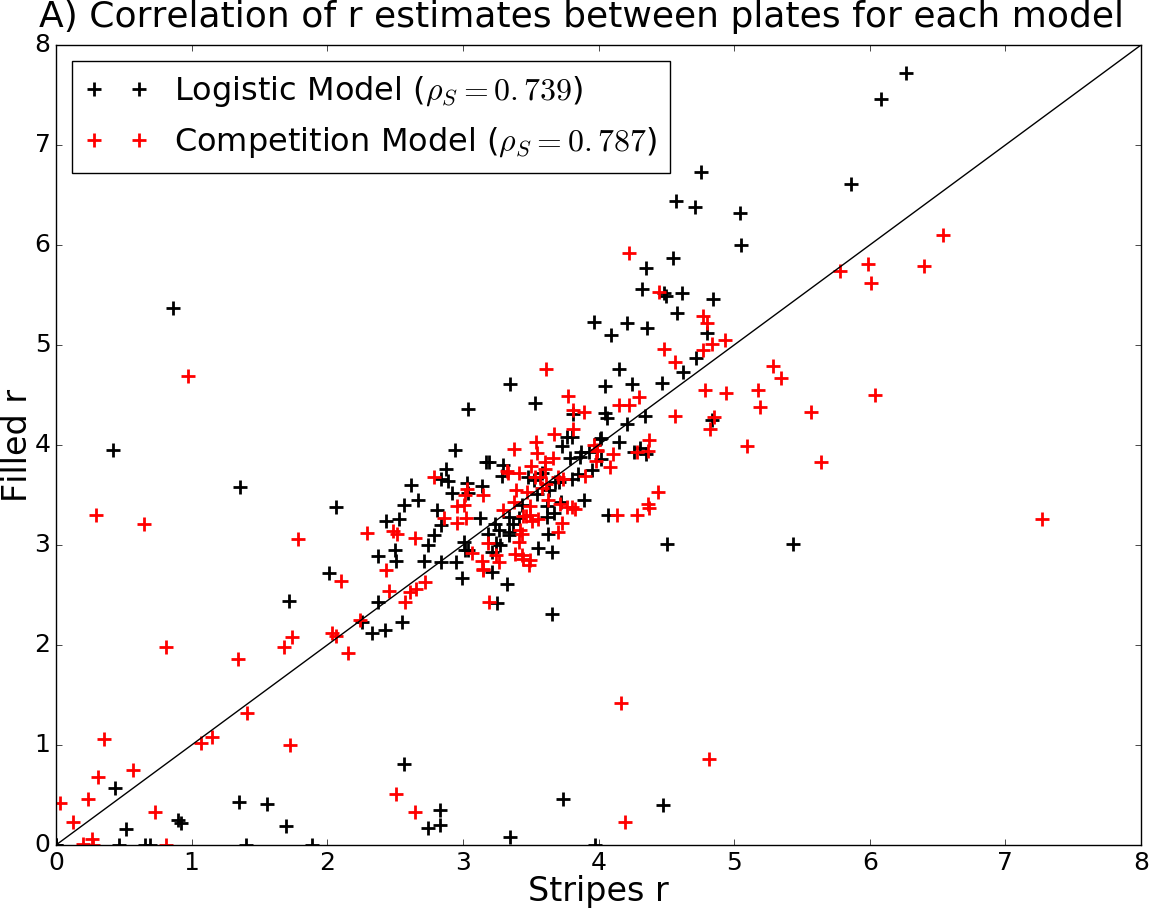
\includegraphics[width=\linewidth]{final/r_correlations_between_plates}
  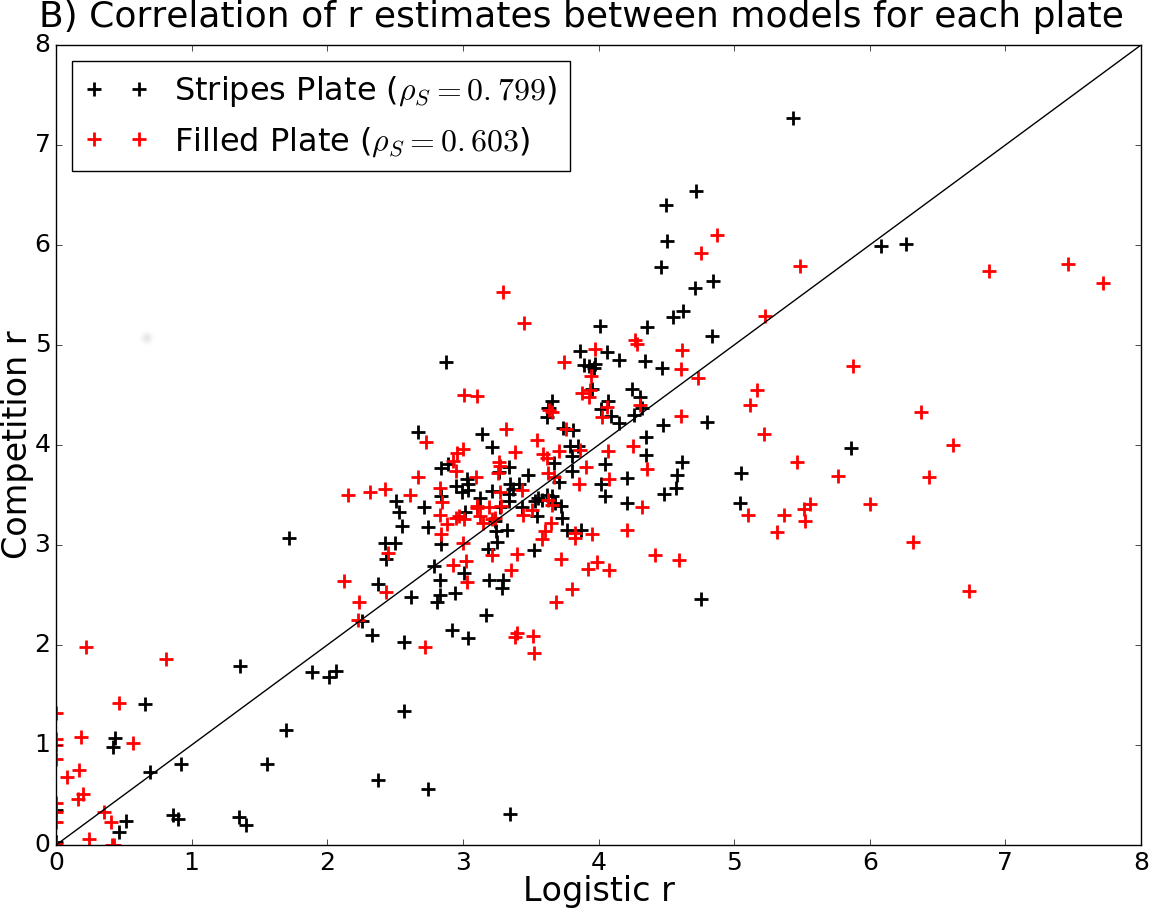
\includegraphics[width=\linewidth]{final/r_correlations_between_models}
  \captionof{figure}{\textbf{Correlation of r estimates for
      ``Stripes'' and ``Filled'' plates.}~I fit the competition model
    and independent model to the ``Stripes'' and ``Filled'' plates in
    Figure~\ref{fig:stripes_images}. I converted competition model b
    to logistic model r. I only used data for cultures that were
    common between the two plates common and removed edge
    cultures. Pearson correlation coefficients, \(\rho\), are shown in
    the legends. The line \(y=x\) is also plotted.}
  \label{fig:r_correlations}
\end{Figure}


\subsection{\thesubsection~Towards a genetic algorithm}

% %\end{multicols}
% \graphicspath{{images/genetic_algorithm/}}
% \begin{Figure}
%   \centering
%   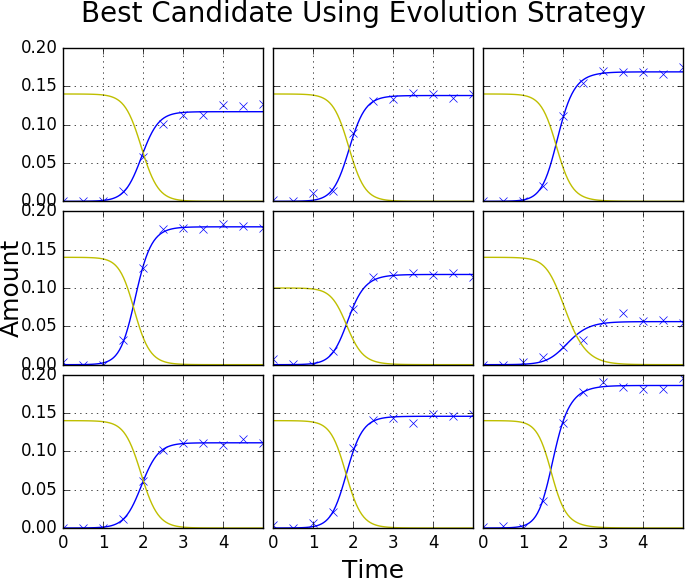
\includegraphics[width=\linewidth]{final/ga_fit_to_sim_true_plate_lvl_trimmed}
%   \captionof{figure}{Genetic algorithm fit to a 3x3 simulation. MIGHT
%     TAKE A LITTLE BIT OF WORK TO REPRODUCE AND COULD USE PARAMETERS
%     FROM THE BEST P15 FIT RATHER THAN JUST PICKING/RANDOMIZING. NEED
%     TO CHECK THAT PLATE LEVEL PARAMETERS WERE ALSO EVOLVED.}
%   \label{fig:3x3_genetic_algorithm_comp_fit_fixed_plate_level}
% \end{Figure}
% %\begin{multicols}{2}


%\end{multicols}
\graphicspath{{images/genetic_algorithm/}}
\begin{Figure}
  \centering
  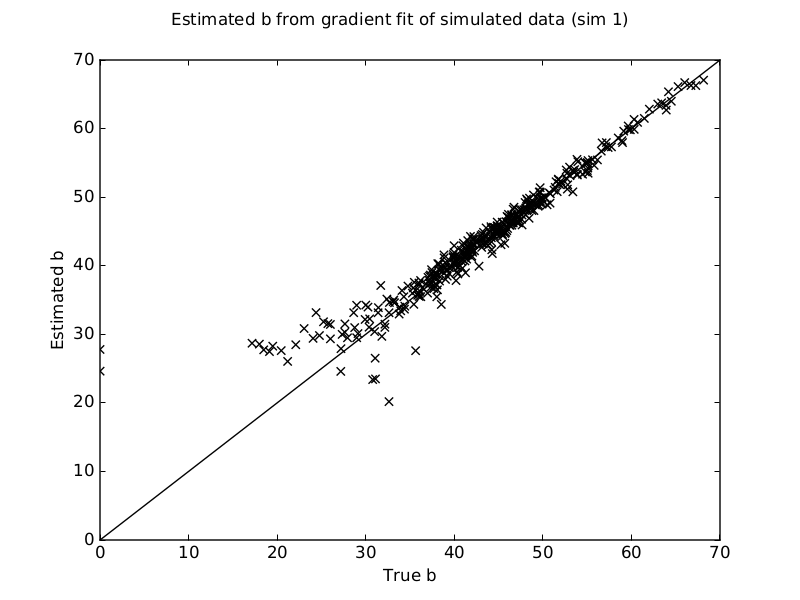
\includegraphics[width=\linewidth]{final/est_b_vs_true_b_imag_neigh_guess_sim_1_trimmed}
  \captionof{figure}{Recovery of true b values from a gradient method
    with fixed plate level parameters. I simulated timecourses from
    the best five competition model fits to p15, fixed the true plate
    level parameters, and used a gradient method to recover b. This
    plot shows the worst case from the five sets of values.}
  \label{fig:comp_fit_fixed_plate_level}
\end{Figure}

% (Currently only have comp obj funs using different cultures (Stripes
% obj fun 0.66) (Filled obj fun 0.76).)


%\begin{multicols}{2}

%%% Local Variables:
%%% mode: latex
%%% TeX-master: "report"
%%% End:
